\begin{table*}[t]
\caption{E4, ladder-censored version: 75{,}730 configurations failed at
$T{=}10$\,s with a numeric prescription and were later recovered on the
ladder. $T_{\min}$ is only known to lie in (previous rung, recovering rung];
the bisection design is still pending. Among the 9{,}902 configurations
unsolved at 80\,s with a numeric prescription, 9{,}594 (96.9\,\%) were prescribed
$T_{\mathrm{req}}>80$\,s, i.e.\ correctly predicted infeasible within the
ladder.}
\label{tab:e4}
\centering\small
\begin{tabular}{lr}
\toprule
recovered no later than the first rung $\ge T_{\mathrm{req}}$ & 91.48\,\% [91.28, 91.68]\\
$T_{\mathrm{req}}/T_{\mathrm{recovered}}$: p5 / p25 / p50 / p75 / p95 &
0.40 / 0.80 / 1.25 / 2.60 / 21.90\\
\bottomrule
\end{tabular}
\end{table*}
\begin{figure}[t]
\centering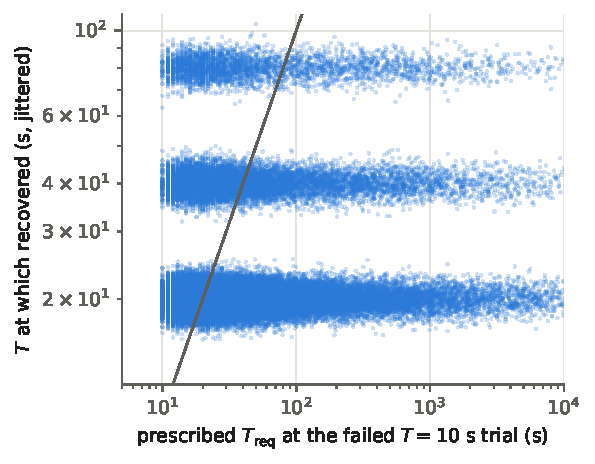
\includegraphics[width=0.75\columnwidth]{figures/E4_prescription.pdf}
\caption{Prescribed $T_{\mathrm{req}}$ against the rung that recovered the
configuration (vertical jitter for visibility); identity line drawn.}
\label{fig:e4}
\end{figure}
